\section{Porównanie laserów}
Analizując pomiary dla 4 laserów które przeprowadziłem, można wyciągnąć nastepujące wnioski:
\begin{itemize}
\item Sprawność różniczkowa  w funkcji zarówno prądu i mocy wejściowej jest większa dla laserów krawędziowych niż dla laserów
 VCSEL, co przedstawia wykres na rysunku ~\ref{fig:plot_eff}.
\item Prąd progowy dla laserów krawędziowych jest większy od prądu progowego dla laserów VCSEL, co przedstawia wykres
na rysunku~\ref{fig:plot_temp_i_th}.
\item Sprawność całkowita w niżsych temperaturach jest większa, zarówno dla laserów VCSEL jak i krawędziowych, co przedstawia
wykres przedstawionym na rysunku~\ref{fig:plot_wall_eff}. Warto zauważyć, że dla laserów krawedziwych wraz z wzrostem prądu
sprawność całkowita spada, dla laserów VCSEL pozostaje ona stała.
\item Tabele 5.5 - 5.8 zawierają porównanie wyznaczonych wartości prądu progowego oraz sprawności z wartościami katalogowymi
firmy Thorlabs. Sprawności się zgadzają. Prąd progowy wyznaczony dla laserów krawędziowych, także zgadza się. Dla laserów VCSEL
wartość prądu progowego jest o 1\,mA za mała. Błąd może być żwiążany z położeniem miernika mocy.
\end{itemize}
\begin{figure}[H]
\center
  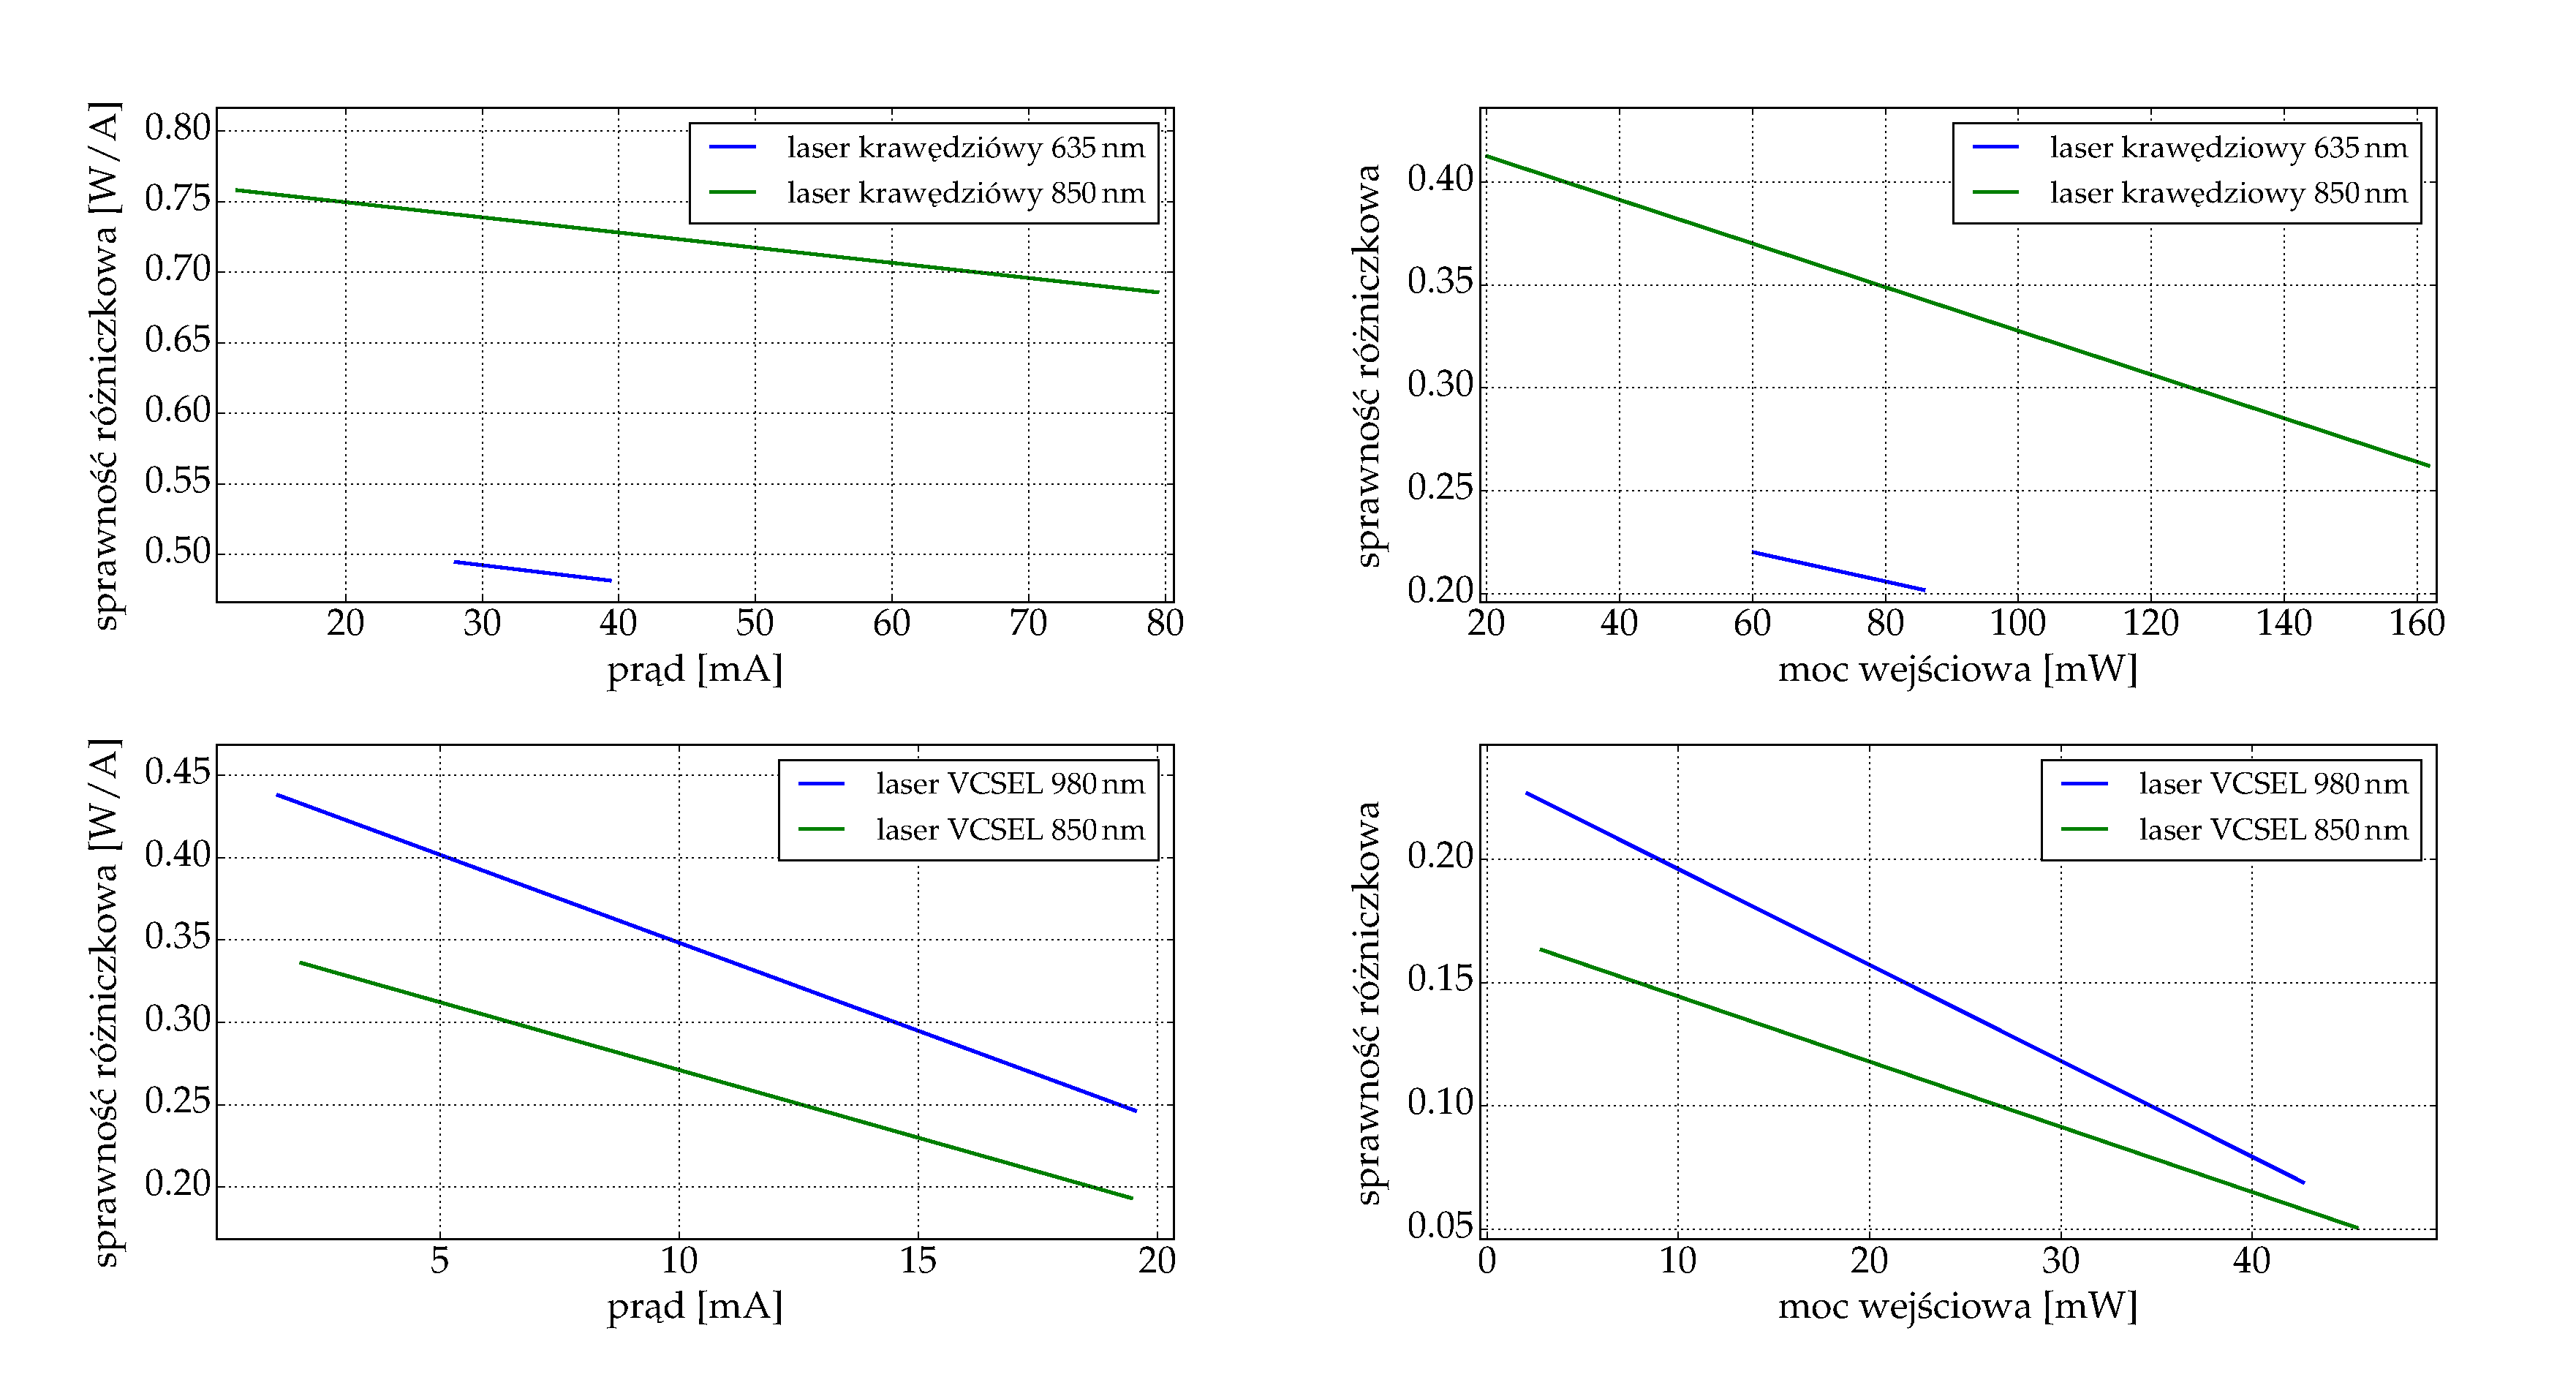
\includegraphics[scale=0.30]{plot_common/plot_eff.eps}
  \caption{Wykres sprawności różniczkowej w funkcji prądu oraz mocy wejściowej w temperaturze 298\,K.}
  \label{fig:plot_eff}
\end{figure}
\begin{figure}
\center
  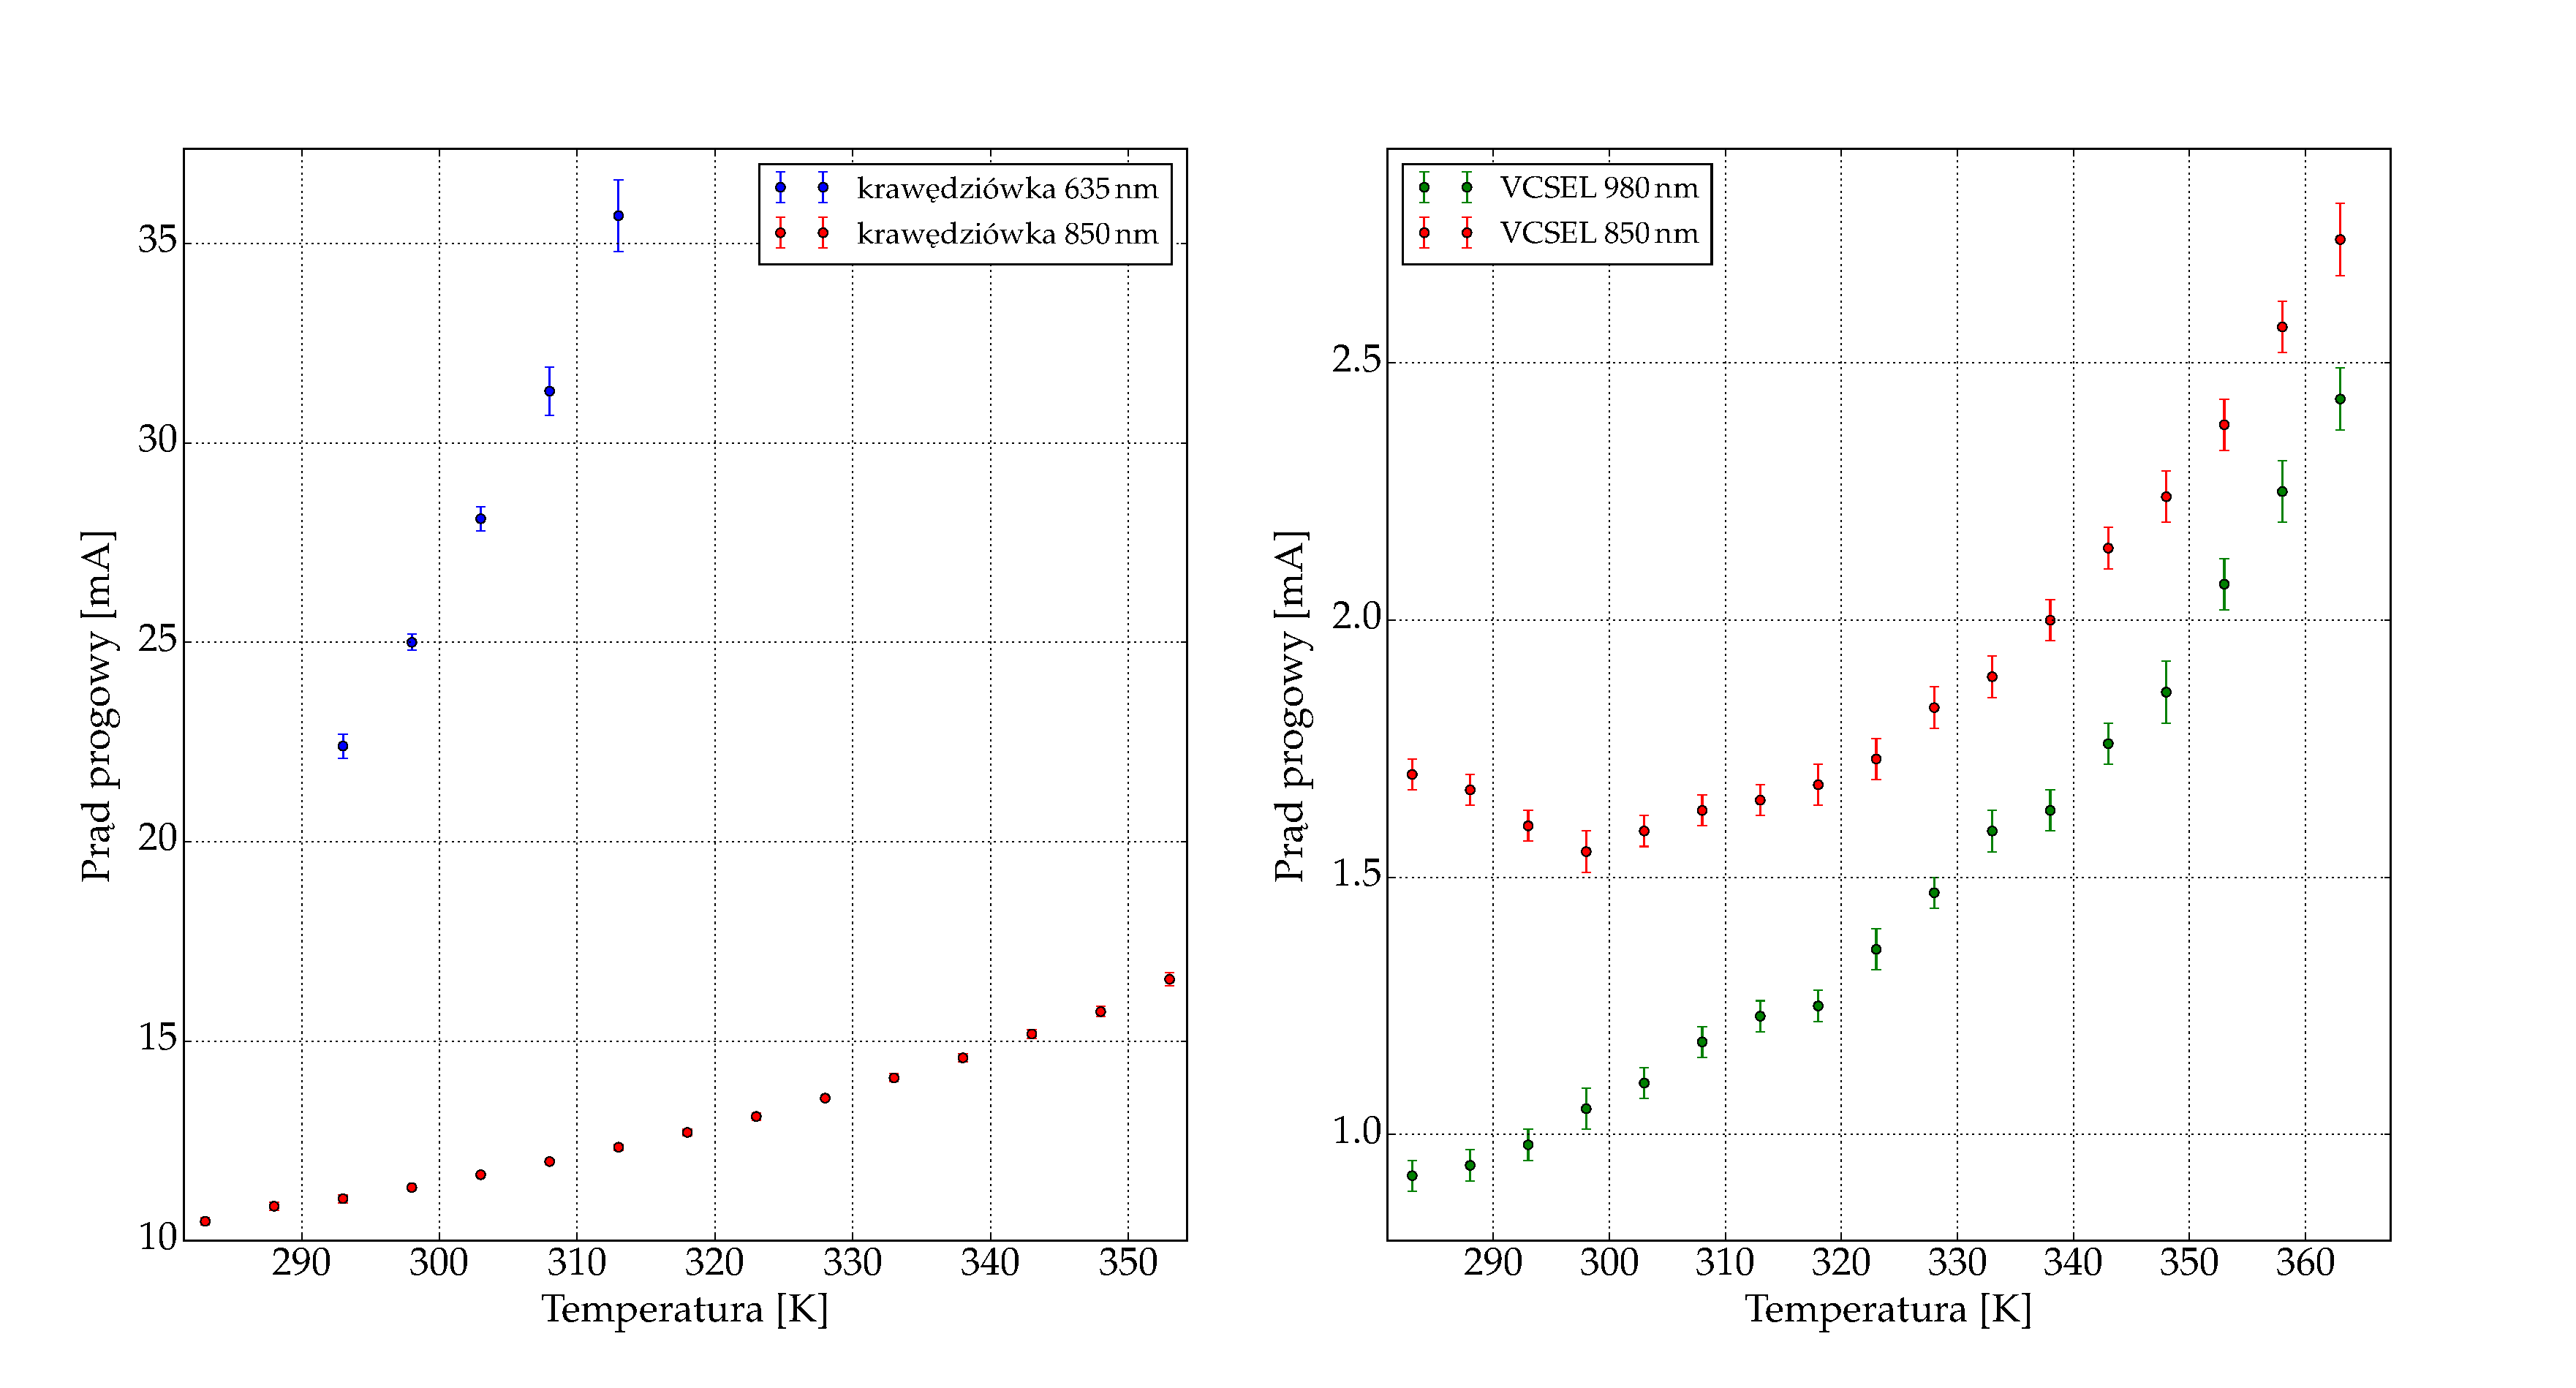
\includegraphics[scale=0.30]{plot_common/plot_temp_i_th.eps}
  \caption{Wykres prądu progowego od temperatury.}
  \label{fig:plot_temp_i_th}
\end{figure}
\begin{figure}
\center
  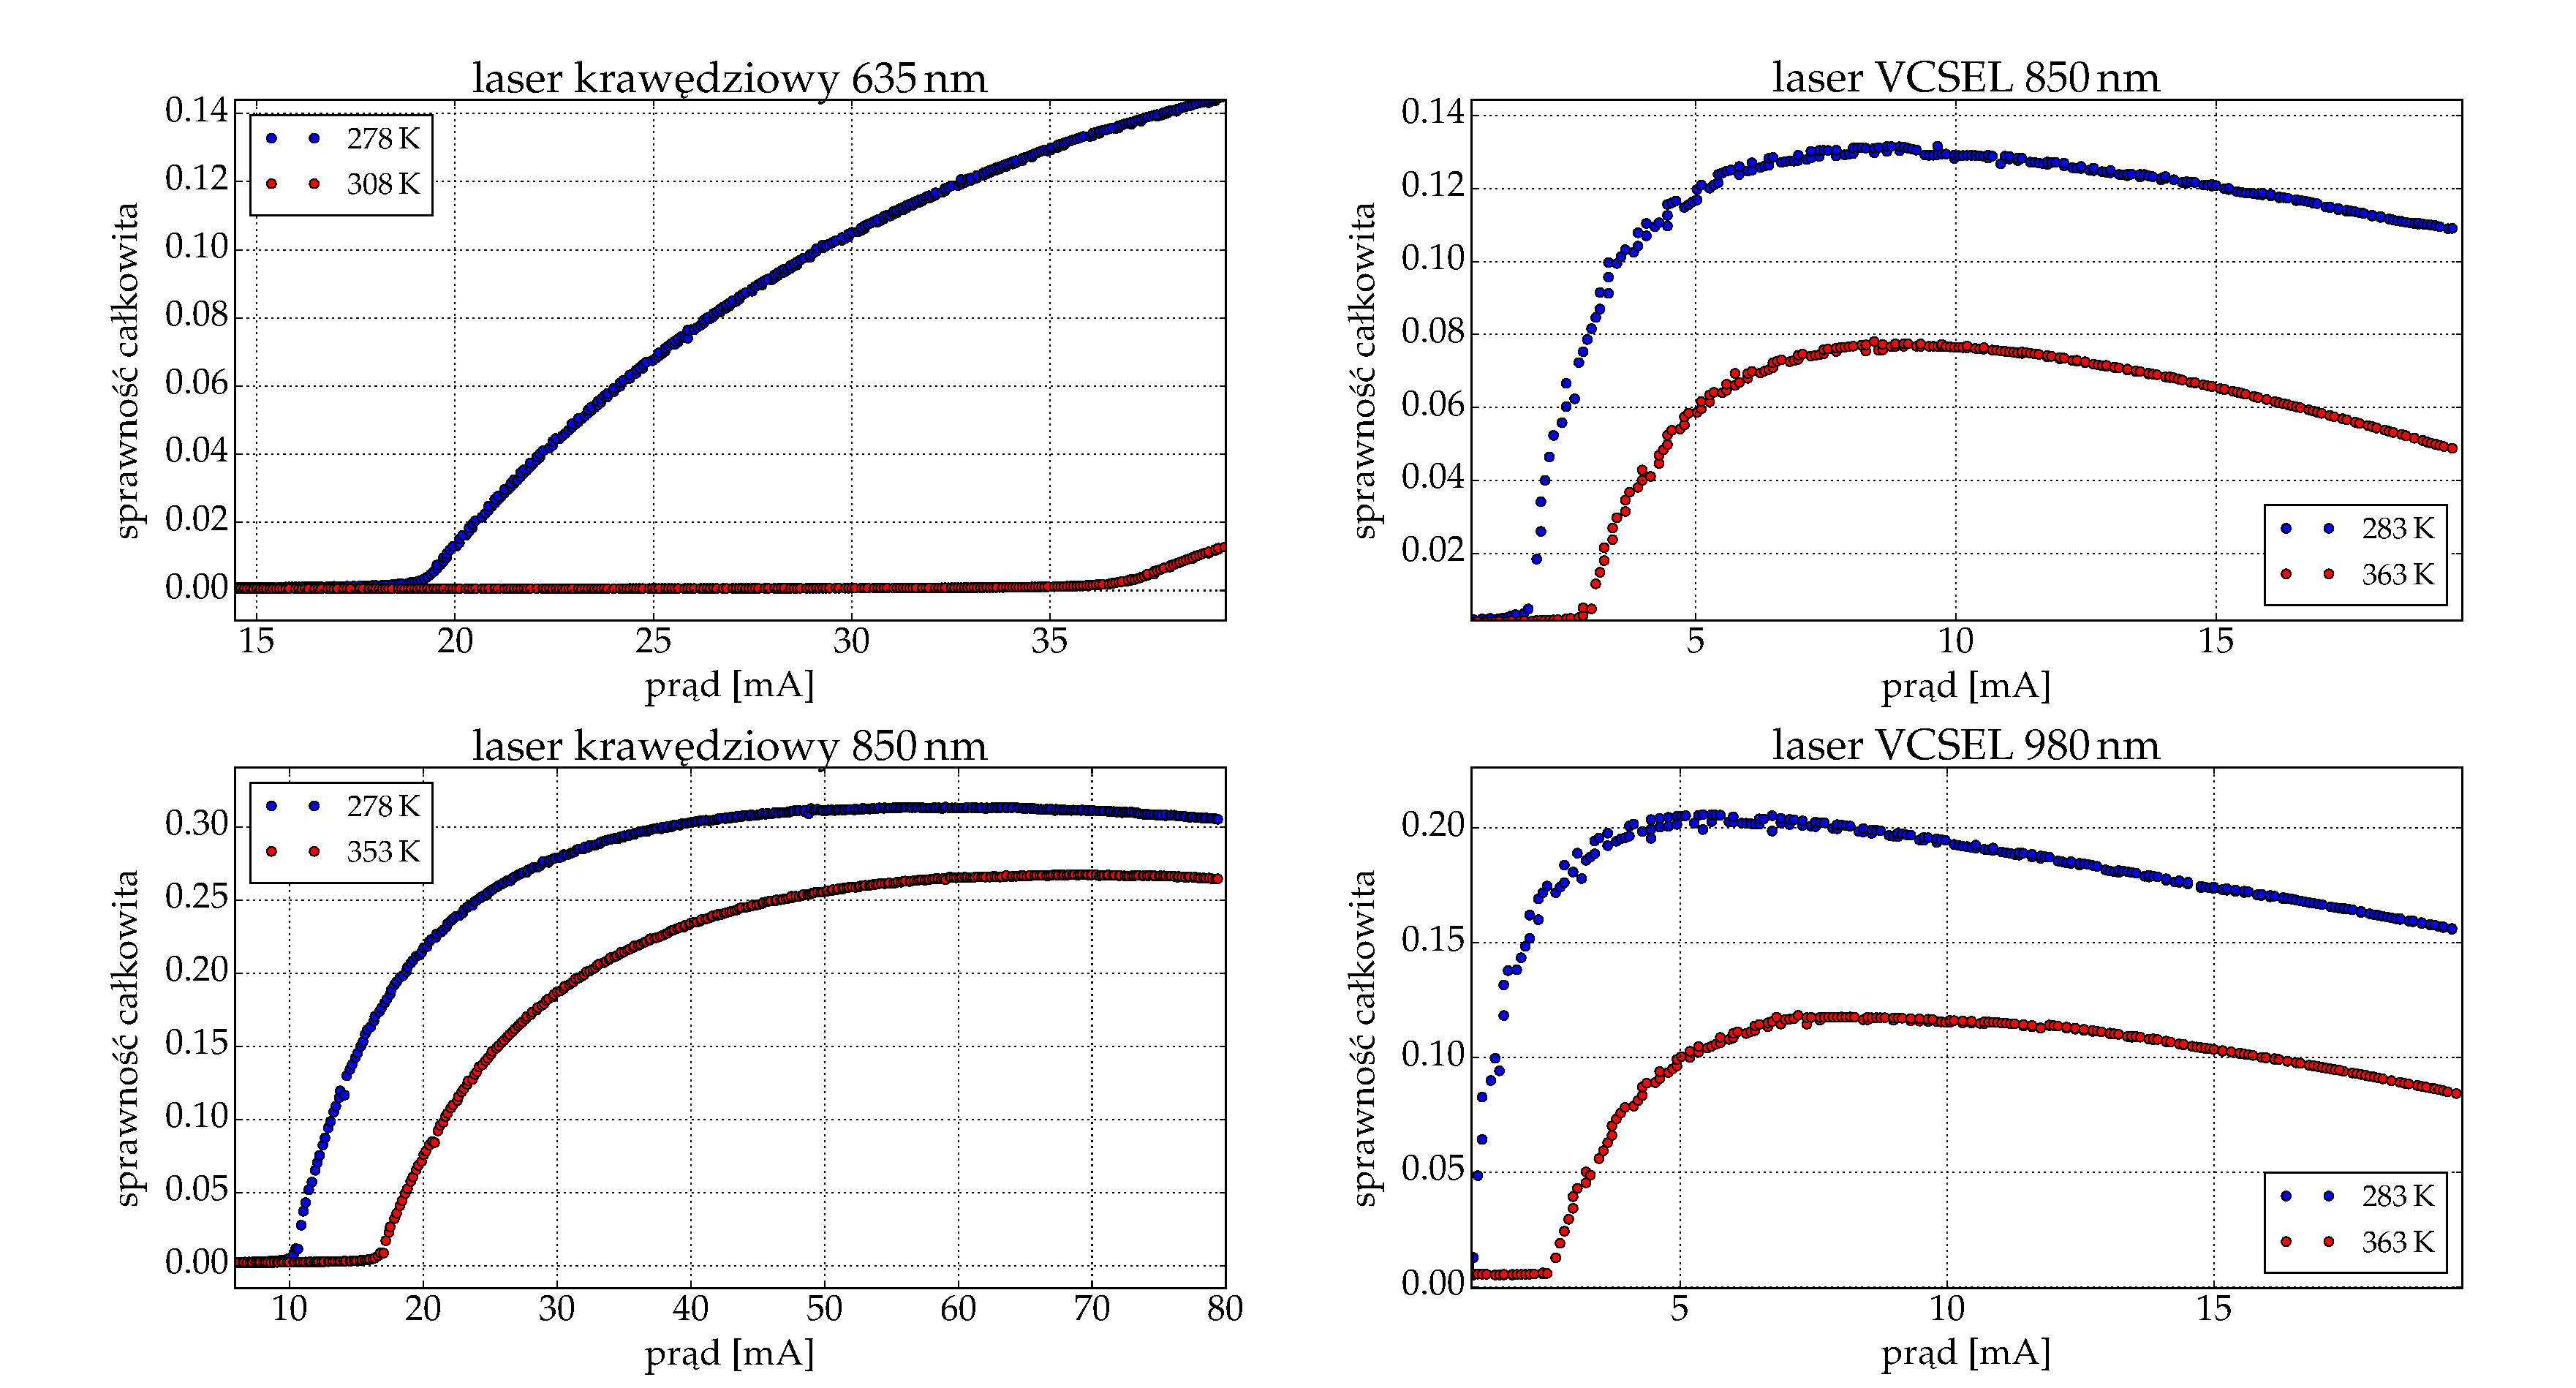
\includegraphics[scale=0.30]{plot_common/plot_wall_eff.eps}
  \caption{Wykres sprawności całkowitej w funkcji prądu.}
  \label{fig:plot_wall_eff}
\end{figure}
\newpage



\begin{table}[h!]
\begin{center}
\label{tab:tabela1}
\caption{Porównanie wartośc prądu progowego oraz sprawności różniczkowej zmierzonego z kartą katologową
 w temperaturze 298\,K dla lasera VCSEL 850\,nm. }
\begin{tabular}{ | C{3.5cm}|  C{1.5cm} | C{1.5cm} | C{1.5cm}| C{3.5cm}|}
\hline
$T$ [K]           &   Min  & typowy & Max   & wyznaczony        \\ \hline
Prąd progowy [mA] &  -    &  2.2    & 3    & 1.55 $\pm$ 0.04  \\ \hline
sprawność [W/A]  przy $I$ = 8\,mA   &  0.12   &  0.32   & 0.4   & 0.28      \\ \hline
\end{tabular}
\end{center}
\end{table}

\begin{table}[h!]
\begin{center}
\label{tab:tabela2}
\caption{Porównanie wartośc prądu progowego oraz sprawności różniczkowej zmierzonego z kartą katologową
 w temperaturze 298\,K dla lasera VCSEL 980\,nm. }
\begin{tabular}{ | C{3.5cm}|  C{1.5cm} | C{1.5cm} | C{1.5cm}| C{3.5cm}|}
\hline
$T$ [K]           &   Min  & typowy & Max   & wyznaczony        \\ \hline
Prąd progowy [mA] &  -    &  2.2    & 3    & 1.05 $\pm$ 0.04  \\ \hline
sprawność [W/A]  przy $I$ = 8\,mA   &  0.12   &  0.32   & 0.4   & 0.37      \\ \hline
\end{tabular}
\end{center}
\end{table}

\begin{table}[h!]
\begin{center}
\label{tab:tabela3}
\caption{Porównanie wartośc prądu progowego oraz sprawności różniczkowej zmierzonego z kartą katologową
 w temperaturze 298\,K dla lasera krawędziowego 850\,nm. }
\begin{tabular}{ | C{3.5cm}|  C{1.5cm} | C{1.5cm} | C{1.5cm}| C{3.5cm}|}
\hline
$T$ [K]           &   Min  & typowy & Max   & wyznaczony        \\ \hline
Prąd progowy [mA] &  10    &  25    & 40    & 11.33 $\pm$ 0.05  \\ \hline
sprawność [W/A]     &  0.3   &  0.5   & 0.7   & 0.49 - 0.48       \\ \hline
\end{tabular}
\end{center}
\end{table}

\begin{table}[h!]
\begin{center}
\label{tab:tabela4}
\caption{Porównanie wartośc prądu progowego oraz sprawności różniczkowej zmierzonego z kartą katologową
 w temperaturze 298\,K dla lasera krawędziowego 635\,nm. }
\begin{tabular}{ | C{3.5cm}|  C{1.5cm} | C{1.5cm} | C{1.5cm}| C{3.5cm}|}
\hline
$T$ [K]           &   Min  & typowy & Max   & wyznaczony        \\ \hline
Prąd progowy [mA] &  -    &  16    & 28    & 27.9 $\pm$ 0.3  \\ \hline
sprawność [W/A]      &  0.4   &  0.6   & 1  & 0.76 - 0.68       \\ \hline
\end{tabular}
\end{center}
\end{table}
